\section{Results}\label{section:eval-results}

The evaluation was conducted during different times of the day. % TODO: count midday, afternoon , evening


TODO persons participated in the evaluation. TODO stated, they identify as male and TODO as female. 
% TODO: evaluate other preliminary questions
% TODO: exmplain studies/work of different users

\subsection{Model Viewer}\label{section:eval-res-mv}

The model viewer experiment, presented in Section~\ref{subsection:model-viewer}, allows users to view \ac{3D} model from different angles. To benchmark extensive usage, a second model instance in another color (the target) is spawned after starting the task. Since in the current implementation, the model cannot be rotated upside down (as mentioned in Section~\ref{subsection:topic-data}), the target is spawned with random reachable orientations.
As soon as the task is started, the user has 30 seconds to match as many orientations as possible. Similar to the implementation by \citeauthor{Katzakis.2010}, the target is rotated to a new random orientation, after one orientation was matched~\cite[140]{Katzakis.2010}.
Because it is hard to match the rotation exactly on all three axes, it is enough to pose the model in a similar orientation to the target. A similar pose is reached, when the smallest angle between the two rotations is less than 20 radians.

\begin{figure}[H]
  \centering
  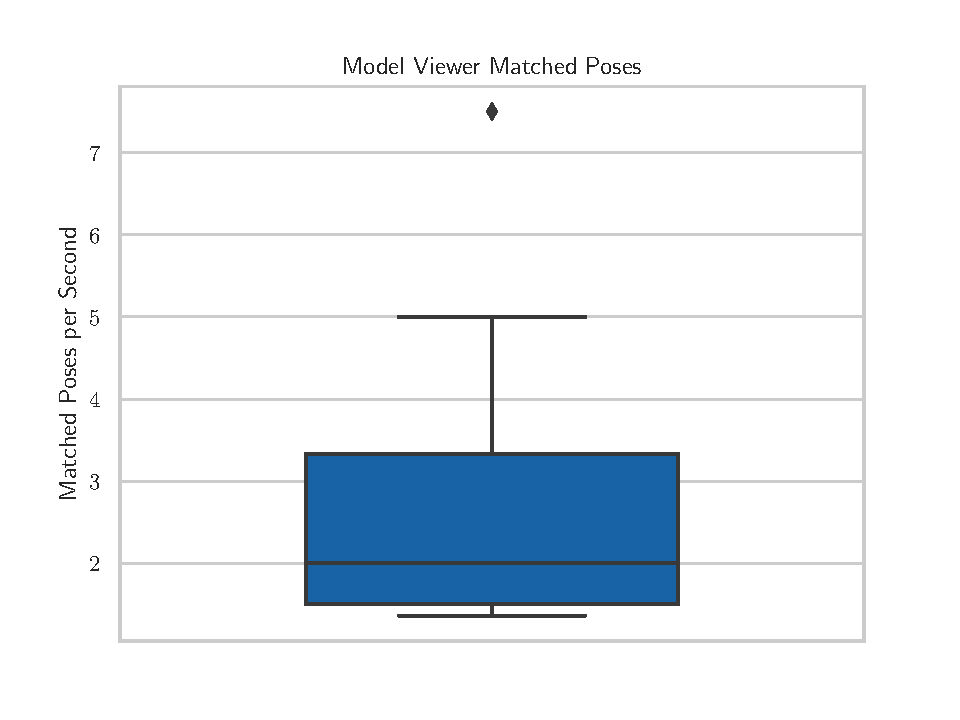
\includegraphics[width=10cm]{figures/evaluation/eval_exp_mv.pdf}
  \caption[Matched poses per second of the model viewer experiment]{A box plot of the time in seconds it took to match a correct pose in the model viewer experiment.}\label{fig:eval-exp-mv}
\end{figure}

% \pgfmathparse{10/6.5}\pgfmathprintnumber[fixed, precision=4]{\pgfmathresult}
\newcommand{\evalExpMvAvgPoses}{3.255} %TODO: correct value
As seen in Figure~\ref{fig:eval-exp-mv}, the average time it took to match a correct poses is roughly \evalExpMvAvgPoses\ seconds. \citeauthor{Katzakis.2010} tracked the time it takes to match a pre-defined pose with a Smartphone, a mouse and a touch panel. The lowest time in average to match one pose, 6.5 seconds, was achieved using the Smartphone as input device~\cite[140]{Katzakis.2010}. This average is significantly higher than the average of this evaluation. This can be due to the fact that users never had to turn the smartphone completely upside down, since rotations were chosen to be always upside up, because of the previously mentioned limitation. Another advantage in the presented implementation is, that the target and the controlled model are not displayed in two separate locations like in {\citetitle{Katzakis.2010}}, but rather with the same origin in the same coordinate space, which makes it easier to see the difference between both rotations~\cite[140]{Katzakis.2010}. Besides the threshold value, also the fact that a skeleton model instead of a multi-colored cube was used, could play a role. 

Nevertheless, 

